% das Papierformat zuerst
%
%\documentclass[a4paper, 11pt,bibtotoc]{scrartcl}
\documentclass[a4paper, 12pt, oneside, final, bibtotoc,abstracton]{scrreprt}  

%\documentclass[
%	a4paper,
%	12pt,
%	oneside,
%	%twoside,
%	%openright,
%	final
%	%draft,				% Entwurf: Druckt keine Bilder
%]{scrreprt}


%F�r URL
\usepackage{url}
\renewcommand{\UrlFont}{\rmfamily}

%F�r Zitaten
\usepackage{cite}

%Abk�rzungen
\usepackage{acronym}


%Inhaltsverzeichnis bearbeiten
\usepackage{tocbibind}

% f�r mathematische Symbole
\usepackage{amsmath}

% tabellen
\usepackage{tabularx}

% Vektorgrafiken mit Latex importieren
\usepackage{import}

\usepackage[colorlinks=false, pdfborder={0 0 0}]{hyperref}
%documentclass[a4paper, 12pt]{article}  
% deutsche Silbentrennung
\usepackage[english,ngerman]{babel}
\renewcommand{\sectfont}{\rmfamily\bfseries}
% wegen deutschen Umlauten
\usepackage[ansinew]{inputenc}
\usepackage{graphicx}
\usepackage{subfigure}\hyphenation{Bit-rate}

%Algorithm schreiben
\usepackage{algorithm2e}

%Tabellen
\usepackage{booktabs}
\usepackage{multirow}
\usepackage{colortbl}


%Farben
\usepackage{xcolor}
\usepackage{color}
\usepackage{listings}%Code einbinden
\definecolor{darkblue}{rgb}{.08,.21,.36}
\definecolor{darkred}{rgb}{.6,.19,.20}
\definecolor{darkgreen}{rgb}{0,.6,0}
\definecolor{red}{rgb}{.98,0,0}
\definecolor{lightblue}{rgb}{0.8,0.85,1}
%\definecolor{lightgrey}{rgb}{0.98,0.98,0.98}
\definecolor{lightgrey}{gray}{.98}
\definecolor{black}{rgb}{0.0,0.0,0.0}


\lstloadlanguages{C++}
\lstset{%
  language=Python,
  basicstyle=\small,
  commentstyle=\itshape\color{darkgreen},
  keywordstyle=\bfseries\color{darkblue},
  stringstyle=\color{darkred},
  showspaces=false,
  showtabs=false,
  columns=fixed,
  backgroundcolor=\color{lightgrey},
  numbers=left,
  frame=single,
  numberstyle=\tiny,
  breaklines=true,
  showstringspaces=false,
  xleftmargin=1cm,
  basicstyle=\small
}%

\usepackage{amssymb}%Mathematische Symbole, wie R,N,Q,Z,...
\setlength{\parindent}{0pt} %einr�cken nach absatz verhindern
%\usepackage{setspace}%Zeilenabstand
\usepackage{algorithmic}%F�r Pseudocode

%%%%%%%%%%%%%%%%%%%%%%%%%%%%%%%%%%%
%Seiten Kopf- und Fu�zeilen
\usepackage[automark,						
		headsepline,								
		plainfootsepline, 
		]{scrpage2}

\automark[section]{chapter} 
\pagestyle{scrheadings}			

\clearscrheadings	%Alte Kopfformatierungen entfernen
\clearscrplain		%Alte Plain-Formatierung entfernen
\clearscrheadfoot %Alten Fu� entfernen
\cfoot[\pagemark]{\pagemark}%Seitenzahl zentriert im Fu� 
\ihead{\leftmark}
\ohead{\rightmark} 


%%%%%%%%%%%%%%%%%%%%%%%%%%%%%% User specified LaTeX commands.

% Mehr Platz zwischen Tabelle und Untertitel
\usepackage{caption}
\captionsetup[table]{skip=10pt}


\colorlet{chapter}{black!75}
\addtokomafont{chapter}{\color{chapter}}
%

%Kapitelzahl sehr gro�
\makeatletter% siehe De-TeX-FAQ 
 \renewcommand*{\chapterformat}{% 
   \begingroup% damit \unitlength-�nderung lokal bleibt 
     \setlength{\unitlength}{1mm}% 
     \begin{picture}(10,10)(0,5) 
       \setlength{\fboxsep}{0pt} 
       %\put(0,0){\framebox(20,40){}}% 
       %\put(0,20){\makebox(20,20){\rule{20\unitlength}{20\unitlength}}}% 
       \put(10,15){\line(1,0){\dimexpr 
           \textwidth-20\unitlength\relax\@gobble}}% 
       \put(0,0){\makebox(10,20)[r]{% 
           \fontsize{28\unitlength}{28\unitlength}\selectfont\thechapter 
           \kern-.05em% Ziffer in der Zeichenzelle nach rechts schieben 
         }}% 
       \put(10,15){\makebox(\dimexpr 
           \textwidth-20\unitlength\relax\@gobble,\ht\strutbox\@gobble)[l]{% 
             \ \normalsize\color{black}\chapapp~\thechapter\autodot 
           }}% 
     \end{picture} % <-- Leerzeichen ist hier beabsichtigt! 
   \endgroup 
}
\makeatother% siehe \makeatletter

\usepackage{ %a4wide,
            ellipsis, fixltx2e, mparhack,   %Fehlerkorrektur f�r Marginalien
            booktabs, longtable             %sch�nere Tabellen
}  

\usepackage{ifpdf} % part of the hyperref bundle
\ifpdf % if pdflatex is used


%set fonts for nicer pdf view
 \IfFileExists{lmodern.sty}{\usepackage{lmodern}}
  {\usepackage[scaled=0.92]{helvet}
    \usepackage{mathptmx}
    \usepackage{courier} }
\fi

%%%%%%%%%%%%%%%%%%%%%%%%%%%%%%%%%%%%%%%%%%%%%%%%%%%%%%%%%%

% sch�nerer Blocksatz!!
\usepackage{microtype}
 
%%%%%%%%%%%%%%%%%%%%%%%%%%%%%%%%%%%

% Hurenkinder und Schusterjungen werden vermieden
\clubpenalty = 10000
\widowpenalty = 10000
\displaywidowpenalty = 10000

%%%%%%%%%%%%%%%%%%%%%%%%%%%%%%%%%%%%%%%%%%%%%%%%%%%%%%%%%%%%%%%%%%%%%
%%% Definitionen
%%%%%%%%%%%%%%%%%%%%%%%%%%%%%%%%%%%%%%%%%%%%%%%%%%%%%%%%%%%%%%%%%%%%%
\begin{filecontents}{cpuAnno.dat}
0 0 5 0.8 20 13.3 35 19.6 50 0.3
\end{filecontents} 
%%%%%%%%%%%%%%%%%%%%%%%%%%%%%%%%%%%%%%%%%%%%%%%%%%%%%%%%%%%%%%%%%%%%%
%%% End Definitionen
%%%%%%%%%%%%%%%%%%%%%%%%%%%%%%%%%%%%%%%%%%%%%%%%%%%%%%%%%%%%%%%%%%%%%


\begin{document}
%\begin{titlepage}
%\begin{center}
%{\huge \textbf{Philipps-Universit�t Marburg}}\\[0.5cm]
%\textbf{Fachbereich 12 - Mathematik und Informatik}\\[0.5cm]
%
%\begin{figure}[h]
%	\centering
%		
\includegraphics[width=0.8\textwidth]{fig/unilogo.pdf}
%\end{figure}
%
%{\huge \textbf{{\large \\[1cm]Masterarbeit}}}
%\\[1cm]
%
%{\huge \textbf{Entwicklung eines interaktiven Editors f�r Flugzeugkonfigurationen ~~~~~~~~~~~~~~ im Vorentwurf}}
%\\[1cm]
%
%{\large von}\\
%{\large Ren\'{e} Frank}\\
%{\large Januar 2015}\\[1.5cm]
%
%{\large
%Betreuer:\\Prof. Dr. Thorsten Thorm�hlen\\[0.5cm]
%Arbeitsgruppe Grafik und Multimedia Programmierung}
%\\[0.8cm]
%{\large
%Betreuer:\\Carsten Liersch\\[0.5cm]Deutsches Zentrum f�r Luft- und Raumfahrt (DLR)\\
%Institut f�r Aerodynamik und Str�mungstechnik}
%
%
%
%
%
%
%
%\end{center}
%\end{titlepage}

%\setstretch {1.15}%Zeilenabstand setzen

  
% hier beginnt das Dokument
\begin{titlepage}
	
\vspace{0.3cm} \noindent\rule{\textwidth}{0.5mm} \vspace{-0.3cm}	
	
%\begin{minipage}{19mm} 
%    %
\includegraphics{fig/siegel_uni.pdf}
%    
\includegraphics{fig/siegel-philipp.eps}
%        
\includegraphics[width=\linewidth]{fig/DLR_Logo.eps}
%\end{minipage}
%	\hfill	
%\begin{minipage}{85mm}	
%	\sffamily
%	%\noindent\Large\textbf{\input{graphics/siegel-philipp.eps}}  
%	
%\begin{flushright}
%	\scriptsize FACHBEREICH MATHEMATIK UND INFORMATIK
%
%	\vspace{0.25cm}
%	
%	\scriptsize Arbeitsgruppe Grafik und Multimedia Programmierung
%\end{flushright}
%
%\end{minipage}	


\begin{minipage}{\linewidth} 
    
\includegraphics{fig/siegel-philipp.eps}
	\hfill	 
    
\includegraphics[scale=0.15]{fig/DLR_Logo}
\end{minipage}

\begin{minipage}{\linewidth}	
	\sffamily
	%\noindent\Large\textbf{\input{graphics/siegel-philipp.eps}}  	
\begin{flushleft}
	\vspace{0.25cm}
		
	\scriptsize FACHBEREICH MATHEMATIK UND INFORMATIK %\hfill Institut f�r Aerodynamik und Str�mungstechnik% DEUTSCHES ZENTRUM F\"UR LUFT- UND RAUMFAHRT%Deutsches Zentrum f�r Luft- und Raumfahrt
	
	\vspace{0.25cm}	

	\scriptsize Arbeitsgruppe Grafik und Multimedia Programmierung \hfill Institut f�r Aerodynamik und Str�mungstechnik 
\end{flushleft}

\end{minipage}	
 
	
%	\noindent\footnotesize Philipps-Universit\"at Marburg,\\
%	\footnotesize Fachbereich 12: Mathematik und Informatik \hfill \today
	\vspace{0.3cm} \noindent\rule{\textwidth}{0.1mm}\vspace{1cm}
	\rmfamily\normalsize	



\begin{center}
\Large{\textsf{\textbf{Entwicklung eines interaktiven Editors f\"ur Flugzeugkonfigurationen im Vorentwurf}}}
 
\vspace{1em}
 
\large{\textsf{Abschlussarbeit zur Erlangung des akademischen Grades}} \\
\Large{\textsf{Master of Science (M.Sc.)}} \\
\large{\textsf{vorgelegt von}}
 
\vspace{0.5em}
 
\textsf{Ren\'{e} Frank B.Sc.}
 
\vspace{5.0em}
 
%\textsf{\makebox[3.5cm][l]{Referentin:}}            \textsf{\makebox[7cm][r]{Prof. Dr. ...}} \\
\textsf{\makebox[3.5cm][l]{Betreuer:}}           \textsf{\makebox[7cm][r]{Prof. Dr. Thorsten Thorm\"ahlen
}} \\
\textsf{\makebox[3.5cm][l]{Betreuer:}}           \textsf{\makebox[7cm][r]{Dipl.-Ing. Carsten Liersch
}}
 

 
 
\textsf{\small{\makebox[3.5cm][l]{Ausgabedatum:}}}  %\textsf{\small{\makebox[7cm][r]{24.05.2012}}}
\textsf{\small{\makebox[7cm][r]{XX.XX.2014}}} \\
 
\textsf{\small{\makebox[3.5cm][l]{Abgabedatum:}}}   %\textsf{\small{\makebox[7cm][r]{01.10.2012}}}
\textsf{\small{\makebox[7cm][r]{XX.XX.2015}}}
\vfill
%\vspace{2cm}


Philipps-Universit\"at Marburg\\
Fachbereich Mathematik und Informatik\\
Hans-Meerwein-Stra\ss e\\
35032 Marburg

\end{center}

\end{titlepage}

\newpage
\shipout\null
\chapter*{Erkl\"arung}
\thispagestyle{empty}

\normalsize
Ich erkl\"are hiermit, dass ich diese Masterarbeit mit dem Titel \textit{Entwicklung eines interaktiven Editors f\"ur Flugzeugkonfigurationen im Vorentwurf} selbstst\"andig ohne Hilfe Dritter und ohne Benutzung anderer als der angegebenen Quellen und Hilfsmittel verfasst habe. Alle den benutzten Quellen w\"ortlich oder sinngem\"a\ss {} entnommenen Stellen sind als solche einzeln kenntlich gemacht.\\

\noindent Diese Arbeit ist bislang keiner anderen Pr\"ufungsbeh\"orde vorgelegt und auch nicht ver\"offentlicht worden.\\

\noindent Ich bin mir bewusst, dass eine falsche Erkl\"arung rechtliche Folgen haben wird.\\[3cm]

 
\vspace{5em}
 
\begin{flushright}
\begin{table}[ht]
\begin{tabularx}{\textwidth}{Xp{7cm}}
%Marburg den \today & \tabularnewline \cline{2-2}  \addlinespace
Marburg den 13.08.12 & \tabularnewline \cline{2-2}  \addlinespace
 & \centering{Ren\'{e} Frank}
\end{tabularx}
\end{table}
\end{flushright}

\begin{abstract}
Viele der in der Computergrafik verwendeten 3D-Modelle werden mit Hilfe der Dreiecksnetze  repr�sentiert. ... (max. 1 Seite)
\end{abstract}

\begin{otherlanguage}{english}
\begin{abstract}
text text text text text text
text text text text
text text text text text text text texttext text
(exakte englische �bersetzung der deutschen Kurzfassung)
\end{abstract}
\end{otherlanguage} 

\newpage
\thispagestyle{empty}
%% Ab jetzt r�mische Seitenzahlen
\pagenumbering{Roman}
\setcounter{page}{0}
\hspace{1cm}
\tableofcontents
\newpage
\pagenumbering{arabic}
\setcounter{page}{1}
\chapter{Einleitung}
Diese Diplomarbeit besch�ftigt sich mit den Parallel View-Dependent Compressed Progressive Meshes und deren Umsetzung in die vom Grafikkartenhersteller NVIDIA entwickelte parallele Programmiersprache CUDA. Dazu geh�rt die Entwicklung einer f�r die parallele Verarbeitung geeignete effiziente Datenstruktur, sowie eine effiziente Datenverwaltung.  

%%%%%%%%%%%%%%%%%%%%%%%%%%%%%%%%%%%%%%%%%%%%%%%%%%%%%%%%%%%%%%%%%%%%%%%%%%%%%%%%%%%
\section{Motivation}
Die aktuelle Entwicklung der Multimediaindustrie versucht zunehmend die Simulation von virtuellen Welten realistisch darzustellen. Die Anspr�che der Anwender werden mit der Zeit immer gr��er und dementsprechend die generierte virtuelle Realit�t immer komplexer. So eine Entwicklung ist unweigerlich mit der  Steigerung der erforderlichen Rechenleistung verbunden, da die simulierten Objekte aus  Millionen von Polygonen bestehen k�nnen und  in Echtzeit dargestellt werden m�ssen.
Im Laufe der Jahre sind viele verschiedene Verfahren entwickelt worden, die das Ziel hatten, die komplexen Objekte mit einem vertretbaren Qualit�tsverlust in Echtzeit darzustellen. Der mit Abstand beste Ansatz, um den Kompromiss zwischen Qualit�t und Geschwindigkeit zu finden, ist die View-Dependent Progressive Meshes. Einer der Vorteile dieser Herangehensweise ist, dass dieses Verfahren hochgradig parallelisierbar ist, so dass sich mit einer geeigneter Programmiersprache und Hardware eine beachtliche Effizienzsteigerung erzielen l�sst.\\
Die von NVIDIA entwickelte parallele Programmiersprache CUDA setzt auf den aktuellen Trend der GPGPUs und  erm�glicht es mit einer kosteng�nstigen Grafikkarte, die in fast jeden Desktoprechner vorhanden ist, Programme effizient zu parallelisieren. Aus diesem Grund ist CUDA f�r das Parallelisieren von View-Dependent Progressive Meshing besonders geeignet.

%%%%%%%%%%%%%%%%%%%%%%%%%%%%%%%%%%%%%%%%%%%%%%%%%%%%%%%%%%%%%%%%%%%%%%%%%%%%%%%%%%%
\section{Ziele}\label{chp:Ziele}   
Das Ziel dieser Arbeit ist die Entwicklung einer effizienten parallelen Implementierung  von komprimierten View-Dependent Progressive Meshes in CUDA, welche in der Lage ist, Objekte die aus mehreren Millionen von Polygonen bestehen k�nnen, in Echtzeit zu verarbeiten.

%%%%%%%%%%%%%
\subsubsection{Echtzeit} 
Das entwickelte Programm soll selbst sehr gro�e Polygonnetze effizient verarbeiten k�nnen. Die Eingaben des Benutzers f�r die Translation und Rotation des Objekts sollen in Echtzeit umgesetzt werden. Die durchschnittliche Laufzeit des Programms pro Frame soll h�chstens drei Mal soviel Zeit wie das Rendering des gegebenen Modells ben�tigen, um eine Echtzeitdarstellung des Modells zu erm�glichen. Dabei k�nnen die Modelle aus mehreren Millionen von Dreiecken bestehen.

%%%%%%%%%%%%%
\subsubsection{Kosten} 
Das Programm sollte mit der normalen, kosteng�nstigen Privatanwender-Hardware laufen, sodass f�r die Ausf�hrung keine Spezialrechner ben�tigt werden. Die einzige Vorrausetzung an das System ist eine NVIDIA-Grafikkarte die CUDA 1.1 unterst�tzt. Diese ist aber in den meisten Desktoprechnern vorhanden oder kann kosteng�nstig nachger�stet werden. 

%%%%%%%%%%%%%%%%%%%%%%%%%%%%%%%%%%%%%%%%%%%%%%%%%%%%%%%%%%%%%%%%%%%%%%%%%%%%%%%%%%%
\section{Aufbau der Arbeit}
Im ersten Abschnitt des Kapitels~\ref{chp:CUDA} soll zun�chst die Bedeutung der Grafikkarte als Berechnungseinheit verdeutlicht werden. Dann soll  im zweiten Abschnitt die Hard- und Softwarearchitektur der Programmiersprache \acs{CUDA} beschrieben werden, sowie einige Vorschl�ge zu Codeoptimierung diskutiert, bevor im Kapitel~\ref{chp:ProgressiveMeshes} ein �berblick �ber die wichtigsten Verfahren zur Echtzeitdarstellung komplexer Objekte geben wird. An dieser Stelle werden auch das View-Dependent Progressive Meshing, sowie einige Simplifizierungstechniken genauer erl�utern.        Kapitel~\ref{chp:ParallelViewDependentRefinementofComprPM} besch�ftigt sich mit der Theorie des im Rahmen dieser Diplomarbeit entwickelten Algorithmus. Dabei sollen die Datenstrukturen, die Kompression, sowie die einzelnen Schritte des Algorithmus genauer erl�utert werden. Die Implementierung des Algorithmus in \acs{CUDA} wird im Kapitel 5 besprochen, dabei sollen die benutzten Bibliotheken, sowie die \acs{CUDA}-spezifische Umsetzung des Programms beschrieben werden. Anschlie�end werden im Kapitel 6 die durchgef�hrten Tests und deren Ergebnisse dokumentiert und diskutiert, sowie im Kapitel 7 ein Ausblick auf weiterf�hrende Arbeiten gegeben. 


%%%%%%%%%%%%%%%%%%%%%%%%%%%%%%%%%%%%%%%%%%%%%%%%%%%%%%%%%%%%%%%%%%%%%%%%%%%%%%%%%%%
\section{Verwandte Arbeiten}
Im  Themenbereich der Progressive Meshes und View-Dependent Progressive Meshes gab es schon am Ende des letzten Jahrzehnts einige  Ver�ffentlichungen \cite{bib:hoppePM, bib:hoppeVPM}.  Diese waren zwar eine gute und notwendige Weiterentwicklung vom klassischen LOD-Algorithmus, erm�glichten aber nicht eine effiziente Echtzeitdarstellung von gro�en Modellen. In \cite{bib:efPM} wurde schlie�lich ein Versuch unternommen eine effizientere Datenstrucktur zu entwickeln, um den Speicherverbrauch zu optimieren und bessere Geschwindigkeit zu erreichen. Diese effizientere Datenstruktur brachte zwar einige Verbesserungen, erm�glichte aber dennoch keine  Echtzeitdarstellung von gro�en Modellen. 
Seit dem gab es eine Reihe von Verfahren, die das Ziel hatten eine effiziente Echtzeitdarstellung von gro�en Modellen zu erm�glichen. Einige von diesen Verfahren nutzten Multi-Triangulationen \cite{bib:DFMP98}, andere Versuchten die  View-Dependent Progressive Meshes weiterzuentwickeln \cite{bib:PAJ01, bib:PD04 ,bib:ESV99}. Doch keins dieser Verfahren konnte die Anforderungen vollst�ndig erf�llen.\\
Eine erst k�rzlich ver�ffentlichte Arbeit \cite{bib:Hoppe2009} machte endlich einen Schritt in die richtige Richtung. Die in dieser Arbeit implementierte GPU-Variante von  parallelen View-Dependent Progressive Meshes erm�glichte eine akzeptable Echtzeitdarstellung von gro�en Modellen. Diese braucht durchschnittlich das dreifache der Zeit, die f�r das Rendering des  Modells ben�tigen wird und l�sst somit einen gro�en Spielraum f�r die Optimierung offen.  

 

%\newpage
%\newpage\thispagestyle{empty}\hspace{1em}\newpage
\chapter{Grundlagen}\label{chp:Grundlagen}
Im Folgenden soll ein \"Uberblick über die in dieser Arbeit verwendeten Technologien gegeben
werden. Eine allgemeine Einf\"uhrung in den Flugzeugentwurfsprozess zeigt anfangs die Einsatzgebiete des SGG-Editors auf.
Weiterhin wird auf das zentrale Datenformat CPACS, auf dem der SGG arbeitet, eingegangen und dessen Aufbau erl\"autert.
Im zweiten Teil werden die dargestellten Flugzeugkomponenten und verwendete Generierungsverfahren vorgestellt.

\section{Flugzeugentwurf}\label{sec:CPACS}
hier steht alles zum Flugzeugentwurfsprozess

\section{CPACS}\label{sec:CPACS}
Wie schon in Kapitel~\ref{sec:CPACS} beschrieben ... steht hier alles zu CPACS

\section{Profile}
Die Form des Querschnitts eines K\"orpers, wird im Folgenden als Profil bezeichnet. In der Aerodynamik ist die Entwicklung und Charakterisierung von Profilen ein wichtiges Teilgebiet. Konstruierte Profile sollen in ihrer Form bestimmten Funktionen gen\"ugen wie beispielsweise die Erzeugung eines dynamischem Auftriebs bei geringem Strömungswiderstand. In Cpacs wird zwischen Rumpf- und Tragfl\"achenprofilen unterschieden. Beide Profiltypen sind unter dem Konten \textit{profiles} als Listen f\"ur x, y und z Koordinaten repr\"asentiert.\\\\

	ooo hier steht ein tikz xml editor\\\\ 

\subsection{Fl\"ugelprofile}
hier steht allgemeines Zeug zu den Profilen

\newcounter{y}
\setcounter{y}{0}

\begin{tikzpicture}
    \foreach \lbl / \fn in {EPPLER 625/e625.dat,
                            WORTMANN FX 2/fx2.dat,
                            EPPLER 664 (EXTENDED)/e664ex.dat,
                            CLARK Y/clarcy.dat,
                            Eiffel 10 (Wright)/eiffel10.dat,
                            FX 69-PR-281/fx69pr281.dat,
                            NACA Munk M-4 airfoil/m4.dat}{
        % Some profiles look better when using plot[smooth]
        \draw[yshift=-\arabic{y}cm,scale=3] node[left=0.5cm] {\lbl}
            plot file{tikz/data/\fn} -- cycle;
        \stepcounter{y}
    }  
\end{tikzpicture}
\footnotetext{Quelle: http://www.texample.net/tikz/examples/airfoil-profiles, Zugriff: 27.10.2014}


\subsubsection{NACA-Serie}
Das National Advisory Committee for Aeronautics oder kurz NACA wurde 1915 gegründet und ist ein direkter Vorg\"anger der US-Bundesbehörde für Luft- und Raumfahrt, NASA. Die NACA war eine amerikanische Organisation, die sich mit der Grundlagenforschung in der Luftfahrt beschäftigte. Eine bedeutende Entwicklung der NACA-Forschungen, sind optimierte Tragf\"achenprofile. Durch aerodynamischen Tests im Windkanal wurde bereits fr\"uh erkannt, dass die Fl\"ugelprofile mit den besten Eigenschaften hinsichtlich Auftriebsbeiwert und Widerstandsbeiwert, viele Gemeinsamkeiten besitzen. NACA-Profile sind somit Variationen eines Ursprungsprofils, die mit Hilfe von analytischen Gleichungen definiert werden. Spezifische Variationen dieses Profils werden durch die Kr\"ummung bzw. Steigung der Skelettlinie sowie die Dicke der Tragfl\"ache oberhalb und unterhalb jener Skelettlinie erzeugt. Im SGG-Editor wurde ein NACA-Generator implementiert, mit dem sich Profile der NACA 4-digit und NACA 5-digit Serie erstellen lassen.

\paragraph{Profile der Vierer-Serie}

In der vierstelligen NACA-Serie ist ein Profil definiert durch:
\begin{itemize}
\item[1.]Ziffer: maximale Profilw\"olbung 
	\begin{itemize}
		\item angegeben in Prozent, bezogen auf die L\"ange der Profilsehne
	\end{itemize}
\item[2.]Ziffer: W\"olbungsrücklage, Position der maximalen Profilw\"olbung
	\begin{itemize}
		\item angegeben in Zehnteln der L\"ange der Profilsehne
	\end{itemize}
\item[3./4.]Ziffer: maximale Profildicke
	\begin{itemize}
		\item angegeben in Prozent, bezogen auf die L\"ange der Profilsehne
	\end{itemize}
\end{itemize} 


Ein symmetrisches NACA 4 Profil kann mit Gleichung \ref{eq:symyt} konstruiert werden. Das Profil ist in seiner Form, nur durch die angegebene Profildicke ver\"andertbar, da die Profilw\"olbung und somit auch dessen Position die Werte Null haben. Gleichung \ref{eq:symyt} enth\"alt Konstanten, die f\"ur eine Profildicke von 20\% vorgesehen sind. Um diese Werte an die jeweils angegebene Profildicke anzupassen, wird die eigentliche Berechung mit $\frac{t}{0.2}$ multipliziert. In Gleichung \ref{eq:symyt} werden zus\"atzlich folgende Parameter verwendet:

\begin{itemize}
	\item[$c$ :] L\"ange der Profilsehne
	\item[$x$ :] Position entlang der Profilsehne auf der Abszissenachse von 0 to c, 
	\item[$y_t$ :] Entfernung der Skelettlinie zur jeweiligen Profilseite an Position x
	\item[$t$ :] Maximale Dicke des Profils multipliziert mit $\frac{1}{100}$
\end{itemize}

\begin{multline}\label{eq:symyt}
y_t= \frac{t}{0.2}c\left[0.2969 \sqrt{\frac{x}{c}} + (-0.1260) \left(\frac{x}{c}\right) + (-0.3516) \left(\frac{x}{c}\right)^2 + 0.2842 \left(\frac{x}{c}\right)^3 \right. \\\left. + (-1.015) \left(\frac{x}{c}\right)^4 \right]
\end{multline}


Soll die trailing edge geschlossen sein, also das Profil an dieser Position eine Dicke gleich Null haben, wird als Koeffizient an der letzen Stelle statt $-1.015$ ein Wert von $-0.1036$ gew\"ahlt.  Es ergeben sich folgende Definitionen f\"ur Ober- und Unterseite des Profils. Die x-Koordinaten sind f\"ur beide Seiten gleich, daher gilt $x_U = x_L = x$. Die y-Koordinaten ebenfalls identisch, nur das diese f\"ur die Oberseite positiv: $y_U = +y_t$ und f\"ur die Unterseite negativ sind: $y_L = -y_t$.\\
Die Generierung eines asymmetrischen NACA 4 Profils braucht zus\"atzlich zu Gleichung \ref{eq:symyt} noch die maximale Profilw\"olbung und die W\"olbungsr\"ucklage, also den Abstand der Profilnase zur maximalen Profilw\"olbung. 

\begin{itemize}
	\item[$m$ :] Maximale W\"olbung multipliziert mit $\frac{1}{100}$
	\item[$p$ :] Position der maximalen W\"olbung multipliziert mit $\frac{1}{10}$ 
	\item[$t$ :] Maximale Dicke des Profils multipliziert mit $\frac{1}{100}$	
\end{itemize}

Mit Gleichung \ref{eq:camber} wird die y-Koordinate der Skelettlinie an einer gegebenen x-Koordinate berechnet. 

\begin{equation}\label{eq:camber}
     y_c = \left\{ \begin{array}{ll} 
     					m \frac{x}{p^2} \left(2p - \frac{x}{c}\right), & 0 \leq x \leq pc \\[0.5cm]
         				m \frac{c-x}{(1-p)^2}\left(1+\frac{x}{c}-2p\right), & pc \leq x \leq c
         			\end{array}\right.
\end{equation}

\vspace{0.5cm}
Die Dicke des gekr\"ummten Fl\"ugelprofils ist senkrecht zur Skelettlinie festgelegt womit f�r Ober- und Unterseite des Profils folgendes gilt:

\begin{equation}
x_U = x - y_t \sin \theta \qquad , \qquad y_U = y_c + y_t \cos \theta
\end{equation}
\begin{equation}
x_L = x + y_t \sin \theta \qquad , \qquad y_L = y_c +-y_t \cos \theta
\end{equation}


$\theta = \arctan \left(\frac{dy_c}{dx}\right)$

\begin{equation}\label{eq:camber}
     \frac{dy_c}{dx} = \left\{ \begin{array}{ll} 
     					\frac{2m}{p^2} \left(p - \frac{x}{c}\right), & 0 \leq x \leq pc \\[0.5cm]
         				\frac{2m}{(1-p)^2}\left(p - \frac{x}{c}\right), & pc \leq x \leq c
         			\end{array}\right.
\end{equation}



text \cite{bib:naca_docu}
\subsubsection{Naca5}

Um den maximalen Auftrieb von Tragfl\"achenprofilen zu erh\"ohen, wurde zus\"atzlich die 5er Naca Serie entwickelt. Ein NACA 5 Profil hat die Form LPQXX (beispielsweise NACA 23009) und wird wie im Folgenden definiert. Hierbei ist zu beachten, dass die ersten beiden Ziffern zur sp\"ateren Berechnung umgrechnet werden.

\begin{enumerate}
	\item Ziffer: Wert zur Berechnung des optimalen Auftriebskoeffizienten bei optimalem Anstellwinkel
		\begin{itemize}
			\item $cl = L * 0.15 $
		\end{itemize}	
	\item Ziffer: Position der gr\"o\ss ten W\"olbung entlang der Sehnenlinie, beginnend bei der leading edge
		\begin{itemize}
			\item $p = P * 5 $
		\end{itemize}
	\item Ziffer: einfache oder gespiegelte Kr\"ummung
		\begin{itemize}
			\item $0$ oder $1$
		\end{itemize}
	\item Ziffer und 5. Ziffer: maximale Dicke in \% zur Sehnenl\"ange
		\begin{itemize}
			\item $t = XX$
		\end{itemize}	
\end{enumerate}

\noindent F\"ur das obige NACA 23009 w\"urde dies folgendes bedeuten: 

\begin{bsp}
NACA 23009
\begin{itemize}
	\item[L] = 2 $\rightarrow$ 2 * 0.15 $\rightarrow$  Auftriebskoeffizient = 0.3
	\item[P] = 3 $\rightarrow$ 3 * 5.0 $\rightarrow$  Position bei = 15\%
	\item[Q] = 0 $\rightarrow$ normale W\"olbung
	\item[XX] = 09 $\rightarrow$ Dicke = 9 \%
\end{itemize}
\end{bsp}

Die Konstruktion eines NACA 5 Profils sieht zwei F\"alle vor. Die ersten beiden Gleichungen beschreiben werden verwendet, wenn das Q gleich 0 ist, also ein Profil mit normaler W\"olbung kontruiert werden soll. Die letzten bewirken im Fall, dass Q gleich 1 ist, eine gespiegelte W\"olbung.\\

W\"olbung (normal)

\begin{equation}
     y_c = \left\{ \begin{array}{ll}
			\frac{k_1}{6}(x^3 - 3mx^2 + m^2 (3-m)x), & 0 \leq x \le m \\[0.5cm]
         		\frac{k_1m^3}{6}(1-x), & m \leq x \leq 1
         	\end{array}\right.
\end{equation}

Anstieg (normal)

\begin{equation}
     \frac{dy_c}{dx} = \left\{ \begin{array}{ll}
					\frac{k_1}{6}(3x^2 - 6mx + m^2 (3-m)), & 0 \leq x \le m \\[0.5cm]
         				-\frac{k_1m^3}{6}, & m \leq x \leq 1
         			\end{array}\right.
\end{equation}

W\"olbung (gespiegelt)

\begin{equation}
     y_c = \left\{ \begin{array}{ll}
			\frac{k_1}{6}\left((x-m)^3 - \frac{k_2}{k_1} (1-m)^3x-m^3x+m^3\right), & 0 \leq x \le m \\[0.5cm]
         		\frac{k_1}{6}\left(\frac{k_2}{k_1}(x-m)^3 - \frac{k_2}{k_1} (1-m)^3 x -m^3x + m^3\right), & m \leq x \leq 1
         	\end{array}\right.
\end{equation}

Anstieg (gespiegelt)

\begin{equation}
     \frac{dy_c}{dx} = \left\{ \begin{array}{ll}
					\frac{k_1}{6}\left(3(x-m)^2 - \frac{k_2}{k_1} (1-m)^3 - m^3\right), & 0 \leq x \le m \\[0.5cm]
         				\frac{k_1}{6}\left(3 \frac{k_2}{k_1} (x-m)^2 - \frac{k_2}{k_1}(1-m)^3 -m^3\right), & m \leq x \leq 1
         			\end{array}\right.
\end{equation}




In Tabelle \ref{tab:naca5} sind die Konstanten m, k1 und k1/k2 definiert. Diese wurden an der Position der maximale W\"olbung bei einem Auftriebsbeiwert von 0.3 bestimmt. Die Ergebnisse f\"ur Anstieg und W\"olbung k\"onnen linear bez\"uglich des gew\"unschten Auftriebsbeitwertes skaliert werden.\\


Das Plotten geschieht mit cosinus
\begin{equation}
     \frac{x_i}{c} = \frac{1}{2} \left[ 1 - \cos \left( \frac{i * \pi}{N-1} \right) \right]
\end{equation}




\begin{table}\label{tab:naca5}
\taburowcolors[2]{white .. black!20}
\centering
\sffamily\footnotesize
\tabulinesep=6pt
\begin{tabu}{|c|c|c|c|c|}
\hline
\rowcolor{RoyalBlue}\color{white}Beschreibung & \color{white}Position max W\"olbung (p) & \color{white}m & \color{white}k1& \color{white}k2/k1 \\
5\% normal &  0.05 & 0.0580 & 361.400 & \\
10\% normal & 0.10 & 0.1260 &  51.640 &\\
15\% normal & 0.15 & 0.2025 &  15.957 & \\
20\% normal & 0.20 & 0.2900 &   6.643 & \\
25\% normal & 0.25 & 0.3910 &   3.230 & \\
10\% gespiegelt & 0.10 & 0.1300 &   51.990 & 0.000764 \\
15\% gespiegelt & 0.15 & 0.2170 &   15.793 & 0.00677 \\
20\% gespiegelt & 0.20 & 0.3180 &   6.520  & 0.0303 \\
25\% gespiegelt & 0.25 & 0.4410 &   3.191 & 0.1355 \\
\hline
\end{tabu}
\caption{NACA 5 Konstanten f\"ur Auftriebskoeffizient von 0.3}
\end{table}








\subsubsection{Skelettlinie}
\begin{algorithm}[H]
 \KwData{bottom profile, top profile, trailing edge, leading edge}
 \KwResult{camber line }
 chord = line from trailing edge to leading edge\;
 \ForEach{p in chord}{
	perp1 = determine perpendicular of chord through point p\;
	\ForEach{p$\_$b in bottom profile}{
		perp2 = determine perpendicular of perp1 through point p$\_$b\;
		determine intersection point of perp1 and perp2\;
		determine distance from intersection point to p$\_$b\;
	}
	dist$\_$b = minimum distance from intersection point to p$\_$b\;
	\ForEach{p$\_$t in top profile}{
		perp2 = determine perpendicular of perp1 through point p$\_$t\;
		determine intersection point of perp1 and perp2\;
		determine distance from intersection point to p$\_$t\;
	}
	dist$\_$t = minimum distance from intersection point to p$\_$t\;	
	get center of dist$\_$t and dist$\_$b
 }
 \caption{Berechnung der Skelettlinie}
\end{algorithm}

\begin{figure}[htpb]
	\centering

\begin{tikzpicture}[scale=1.3]
\draw[dashed] (0,0)  -- (11,0) node[anchor=west] {};
\draw[] (7.0,-2) -- (7,3.5) node[anchor=south] {};
\draw[] (9.5,1.2) -- (1.0,1.2) node[anchor=south] {};
\draw[color=red] (1.9,1.2) circle (4pt);
\draw[color=red] (7.0,1.2) circle (4pt);
\draw (7.6,3.3) node {\scriptsize Normale 1};
\draw (4.0,1.0) node {\scriptsize Normale 2};

\draw (9.0,-0.2) node {\scriptsize Profilsehne};
\draw (1.7,1.45) node {\scriptsize p$\_$t};
\draw (7.75,0.9) node {\scriptsize Schnittpunkt};

% camber line    
\draw[smooth, scale=11] plot coordinates {(1.000000,-0.001260)(0.998459,-0.000891)(0.993844,0.000204)(0.986185,0.001995)(0.975528,0.004429)(0.961940,0.007435)(0.945503,0.010922)(0.926320,0.014786)(0.904508,0.018907)(0.880203,0.023155)(0.853553,0.027393)(0.824724,0.031479)(0.793893,0.035273)(0.761249,0.038641)(0.726995,0.041457)(0.691342,0.043611)(0.654508,0.045011)(0.616723,0.045586)(0.578217,0.045292)(0.539230,0.044113)(0.500000,0.042060)(0.460770,0.039175)(0.421783,0.035527)(0.383277,0.031213)(0.345492,0.026354)(0.308658,0.021088)(0.273005,0.015572)(0.238751,0.009973)(0.206107,0.004464)(0.175276,-0.000779)(0.146447,-0.005583)(0.119797,-0.009784)(0.095492,-0.013227)(0.073680,-0.015770)(0.054497,-0.017286)(0.038060,-0.017667)(0.024472,-0.016822)(0.013815,-0.014677)(0.006156,-0.011179)(0.001541,-0.006292)(0.000000,0.000000)(0.000000,0.000000)(0.001541,0.007462)(0.006156,0.015828)(0.013815,0.025031)(0.024472,0.034965)(0.038060,0.045492)(0.054497,0.056447)(0.073680,0.067641)(0.095492,0.078871)(0.119797,0.089923)(0.146447,0.100583)(0.175276,0.110640)(0.206107,0.119892)(0.238751,0.128156)(0.273005,0.135268)(0.308658,0.141087)(0.345492,0.145503)(0.383277,0.148432)(0.421783,0.149823)(0.460770,0.149656)(0.500000,0.147940)(0.539230,0.144718)(0.578217,0.140058)(0.616723,0.134060)(0.654508,0.126846)(0.691342,0.118564)(0.726995,0.109382)(0.761249,0.099488)(0.793893,0.089083)(0.824724,0.078383)(0.853553,0.067607)(0.880203,0.056983)(0.904508,0.046736)(0.926320,0.037085)(0.945503,0.028238)(0.961940,0.020390)(0.975528,0.013714)(0.986185,0.008359)(0.993844,0.004445)(0.998459,0.002061)(1.000000,0.001260)};    	
\end{tikzpicture}

	\caption{Berechnung eines Punktes der Skelettlinie}
	\label{fig:airfoil_chamber_algorithm}
\end{figure}



\subsubsection{Sonstiges}

\begin{figure}[htpb]
	\centering
\beginpgfgraphicnamed{profile-f1}
\footnotesize
\begin{tikzpicture}[>=latex,scale=1.11]
\tikzstyle{spring}=[snake=zigzag,thick,line before snake=0.3cm,line after  snake=0.3cm,segment length=6,segment amplitude=5,join=round]%
\begin{scope}[rotate around={-13:(10,0)}]
% bottom_second
\draw[smooth,line width=1pt] plot coordinates {(0,0)(0.0334,-0.0767)(0.1087,-0.1437)(0.2253,-0.2011)(0.3824,-0.2489)(0.5790,-0.2870)(0.8139,-0.3158)(1.0860,-0.3355)(1.3940,-0.3466)(1.7365,-0.3497)(2.1123,-0.3457)(2.5199,-0.3356) (2.9580,-0.3209)(3.4252,-0.3029)(3.9198,-0.2835)(4.4427,-0.2625)(4.9936,-0.2377)(5.5666,-0.2102)(6.1594,-0.1810)(6.7696,-0.1513)(7.3950,-0.1217)(8.0332,-0.0930)(8.6815,-0.0653)(9.3376,-0.0386)(9.9988,-0.0125)};
% top_first
\draw[smooth,line width=1pt,fill=black!5] plot coordinates {(0,0)(0.0095,0.0831)(0.0624,0.1691)(0.1590,0.2574)(0.2990,0.3467)(0.4824,0.4357)(0.7085,0.5225)(0.9765,0.6050)(1.2855,0.6812)(1.6341,0.7488)(2.0206,0.8055)(2.4433,0.8492)(2.8998,0.8778)(3.3879,0.8897)(3.9049,0.8833)(4.4459,0.8592)(5.0064,0.8210)(5.5876,0.7687)(6.1870,0.7023)(6.8016,0.6219)(7.4286,0.5277)(8.0650,0.4197)(8.7080,0.2980)(9.3544,0.1623)(10.0012,0.0125)};
% sekelett
\draw[dashed, color=red, line width=0.5pt] plot coordinates { (0.0, 0.0)(0.021, 0.003)(0.086, 0.013)(0.192, 0.028)(0.341, 0.049)(0.531, 0.074)(0.761, 0.103)(1.031, 0.135)(1.34, 0.167)(1.685, 0.2)(2.066, 0.23)(2.482, 0.257)(2.929, 0.278)(3.407, 0.293)(3.912, 0.3)(4.444, 0.298)(5.0, 0.292)(5.577, 0.279)(6.173, 0.261)(6.786, 0.235)(7.412, 0.203)(8.049, 0.163)(8.695, 0.116)(9.346, 0.062)(10.0, 0.0) };
\draw[line width=0.5pt,dashed,dash pattern=on 4pt off 1.5pt,rotate around={13:(3,0)}](-1,0)--(3,0);
% arrows
\draw[line width=0.5pt,<-](3,0) +(180:3.5cm) arc (180:193:3.5cm);
\draw(3,0) +(186.5:3.7cm) node{$\alpha$};
% sehne
\draw[line width=0.5pt,color=red, dashed,dash pattern=on 4pt off 1.5pt](0,0)--(9.8,0);
\end{scope}%
\end{tikzpicture}
\endpgfgraphicnamed%



\begin{tikzpicture}
% profile with data file
%\newcounter{y}
\setcounter{y}{0}
\foreach \x in {1.00}
    \draw (11 cm,1pt) -- (11 cm,-1pt) node[anchor=north] {$\x$};
    \draw (1pt,0 cm) -- (-1pt,0 cm) node[anchor=east] {$0$};
	\draw (1pt,1.25 cm) -- (-1pt,1.25 cm) node[anchor=east] {$0.10$};
	\draw (1pt,-1.25 cm) -- (-1pt,-1.25 cm) node[anchor=east] {$-0.10$};
    \foreach \lbl / \fn in {naca4815.dat}{
        % Some profiles look better when using plot[smooth]
        \draw[yshift=-\arabic{y}cm,scale=11, fill=black!5]% node[left=0.5cm] {\lbl}
            plot file{tikz/data/\fn} -- cycle;
        \stepcounter{y}
    }
% axis
\draw[thick,-] (0,0)  -- (12,0) node[anchor=west] {x};
\draw[thick,-] (0,-2) -- (0,2) node[anchor=south] {y};    
% camber line    
\draw[smooth, dashed, scale=11] plot coordinates {(1.0,0.0)(0.998459,0.000614)(0.993844,0.0024245)(0.986185,0.0053355)(0.975528,0.00919)(0.96194,0.0137755)(0.945503,0.018829)(0.92632,0.0240435)(0.904508,0.029078)(0.880203,0.0335675)(0.853553,0.037132)(0.824724,0.039389)(0.793893,0.0399975)(0.761249,0.0399065)(0.726995,0.039667)(0.691342,0.039262)(0.654508,0.038677)(0.616723,0.037901)(0.578217,0.036926)(0.53923,0.03575)(0.5,0.034375)(0.46077,0.0328075)(0.421783,0.0310595)(0.383277,0.0291465)(0.345492,0.0270885)(0.308658,0.0249115)(0.273005,0.022642)(0.238751,0.0203125)(0.206107,0.0179555)(0.175276,0.0156075)(0.146447,0.013304)(0.119797,0.0110825)(0.095492,0.008979)(0.07368,0.0070285)(0.054497,0.005264)(0.03806,0.0037155)(0.024472,0.0024095)(0.013815,0.0013695)(0.006156,0.000613)(0.001541,0.000154)(0.0,0.0)};    	
\end{tikzpicture}    


\begin{tikzpicture}
% axis
\draw[thick,-] (11,0)  -- (12,0) node[anchor=west] {x};
\draw[thick,-] (0,-2) -- (0,2) node[anchor=south] {y};
% profile with data file
%\newcounter{y}
\setcounter{y}{0}
\foreach \x in {1.00}
    \draw (11 cm,1pt) -- (11 cm,-1pt) node[anchor=north] {$\x$};
    \draw (1pt,0 cm) -- (-1pt,0 cm) node[anchor=east] {$0$};
	\draw (1pt,1.25 cm) -- (-1pt,1.25 cm) node[anchor=east] {$0.10$};
	\draw (1pt,-1.25 cm) -- (-1pt,-1.25 cm) node[anchor=east] {$-0.10$};
    \foreach \lbl / \fn in {naca4815.dat}{
        % Some profiles look better when using plot[smooth]
        \draw[yshift=-\arabic{y}cm,scale=11]% node[left=0.5cm] {\lbl}
            plot file{tikz/data/\fn} -- cycle;
        \stepcounter{y}
    }
% camber line    
\draw[smooth, dashed, color=red, scale=11] plot coordinates {(1.0,0.0)(0.998459,0.000614)(0.993844,0.0024245)(0.986185,0.0053355)(0.975528,0.00919)(0.96194,0.0137755)(0.945503,0.018829)(0.92632,0.0240435)(0.904508,0.029078)(0.880203,0.0335675)(0.853553,0.037132)(0.824724,0.039389)(0.793893,0.0399975)(0.761249,0.0399065)(0.726995,0.039667)(0.691342,0.039262)(0.654508,0.038677)(0.616723,0.037901)(0.578217,0.036926)(0.53923,0.03575)(0.5,0.034375)(0.46077,0.0328075)(0.421783,0.0310595)(0.383277,0.0291465)(0.345492,0.0270885)(0.308658,0.0249115)(0.273005,0.022642)(0.238751,0.0203125)(0.206107,0.0179555)(0.175276,0.0156075)(0.146447,0.013304)(0.119797,0.0110825)(0.095492,0.008979)(0.07368,0.0070285)(0.054497,0.005264)(0.03806,0.0037155)(0.024472,0.0024095)(0.013815,0.0013695)(0.006156,0.000613)(0.001541,0.000154)(0.0,0.0)};  
% sehne
\draw[line width=0.5pt,color=red](0,0)--(11,0);    	
\end{tikzpicture} 
	\caption{Eine Vektorgrafik}
	\label{fig:vectorExample}
\end{figure}










\subsection{Rumpfprofile}
\blindtext






%\newpage
%\newpage\thispagestyle{empty}\hspace{1em}\newpage
\chapter{Eigenes Verfahren}
In diesem Kapitel soll das eigene Verfahren beschrieben werden. Es geht dabei nicht nur darum zu beschreiben was gemacht wurde, sondern ebenfalls darum zu begr�nden, weshalb bestimmte Design-Entscheidungen getroffen wurden.


\section{LaTex-Editoren}

Ein guter Cross-Plattform (Windows/Linux/Mac) Latex-Editor mit englischer und deutscher Rechtschreibkorrektur ist z.B. TexStudio
(\url{http://texstudio.sourceforge.net/}). Unter Windows verwende ich diesen Editor gerne zusammen mit dem Sumatra PDF Viewer (\url{http://blog.kowalczyk.info/software/sumatrapdf/free-pdf-reader.html}), da dieser ein automatisches Neuladen unterst�tzt.

%%%%%%%%%%%%%%%%%%%%%%%%%%%%%%%%%%%%%%%%%%%%%%%%%%%%%%%%%%%%%%%%%%%%%%%%%%%%%%%%%%%%%%%%%%%%%%%%%%%%%%%%%%%%%%%%%%%%%%%%%
\section{Beispiel f�r eine Tabelle}
In Tabelle \ref{tab:bibliotheken} sind die verwendeten Bibliotheken ausgelistet.
\begin{table}[htbp]
\centering 
\begin{tabular}{ll}
\toprule \textbf{Bibliothek} & \textbf{Version} \\
\bottomrule
CUDA SDK & 2.3 \\
CUDA Toolkit & 2.3 \\
 OpenGL & 3.2 \\
 GLUT & 3.7 \\
GLEW & 1.5.1 \\
CUDPP & 1.1 \\
\bottomrule
\end{tabular}
\caption{Die verwendeten Bibliotheken.}
\label{tab:bibliotheken}
\end{table}

\section{Formel in Latex und Konventionen zur Verwendung mathematischer Symbole}
Mathematische Symbole k�nnen in Latex sehr leicht erzeugt werden. Beispiel f�r Symbole im Text: Gegeben sei ein Skalar $a \in \mathbb{R}$. Tabelle~\ref{tab:mathematischeSymbole} liste einige Konventionen zur Verwendung mathematischer Symbole. Abgesetzte Formel lassen sich ebenfalls leicht erzeugen:
\begin{equation}
\label{eqn:beispiel}
f(x) = x^2 + 3
\end{equation}
Au�erdem kann leicht auf abgesetzte Formel verwiesen werden (siehe Gleichung~\ref{eqn:beispiel}). F�r mehrere ausgerichtete Formeln bietet sich die Umgebung \texttt{eqnarray} an:
\begin{eqnarray}
\label{eqn:beispiel2}
f(x) &=& x^2 + 3 \\
g(\theta) &=& \cos (2\theta) = \cos^2 \theta - \sin^2 \theta\\
h(x) &=& \int_0^\infty \mathrm{e}^{-x}\,\mathrm{d}x
\end{eqnarray}


\begin{table}[htbp]
\centering
\begin{tabular}{lll}
\toprule \textbf{Typ} & \textbf{Schriftart} & \textbf{Beispiele} \\
\bottomrule
Variablen (Skalare) & kursiv & $a, b, x, y$ \\
Funktionen & aufrecht& $\mathrm{f}, \mathrm{g}(x), \mathrm{max}(x)$\\
Vektoren & fett, Elemente zeilenweise & $\mathbf{a}, \mathbf{b}= \begin{pmatrix}x\\y\end{pmatrix} = (x, y)^\top$\\
Matrizen & Schreibmaschine& $\mathtt{A}, \mathtt{B}= \begin{bmatrix}a & b\\c & d\end{bmatrix}$\\
Mengen & kalligrafisch& $\mathcal{A}, \{a, b\} \in \mathcal{B}$ \\
Zahlenbereiche & doppelt gestrichen& $\mathbb{N}, \mathbb{Z}, \mathbb{R}^2, \mathbb{R}^3$ \\
\bottomrule
\end{tabular}
\caption{Konventionen zur Verwendung mathematischer Symbole}
\label{tab:mathematischeSymbole}
\end{table}






\section{Beispiel f�r eine Vektorgrafik}

Wenn m�glich sollten immer Vektorgrafiken verwendet werden. Rastergrafiken sollten nur dann eingesetzt werden, wenn die Original-Quelle ebenfalls eine Rastergrafik ist. Ein 
Cross-Plattform Editor zur Erstellung von Vektorgrafiken ist z.B. Inkscape:
\url{http://inkscape.org/download/}. Nach der Erstellung in Inkscape sollte die Grafik zum einen zur sp�teren Weiterverarbeitung als SVG gespeichert werden. Zum anderen zwecks Import in Latex als PDF. Abbildung~\ref{fig:vectorExample} zeigt ein Beispiel.


\begin{figure}[htpb]
	\centering
		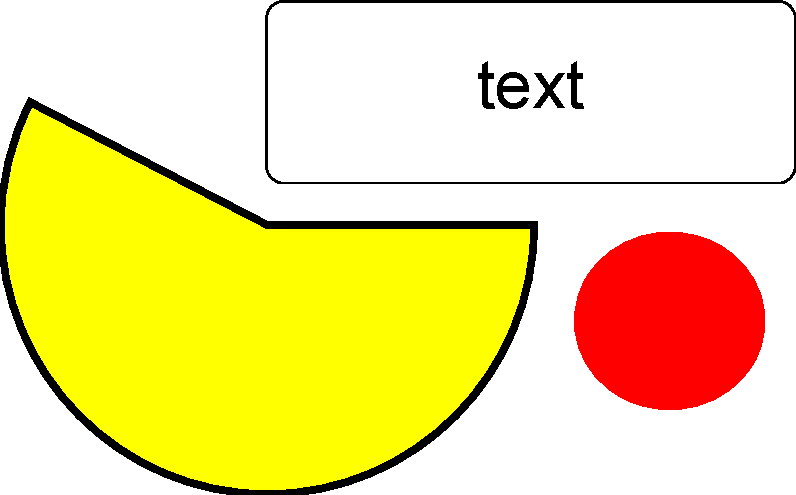
\includegraphics[width=0.30\textwidth]{fig/vectordrawing.pdf}
	\caption{Eine Vektorgrafik}
	\label{fig:vectorExample}
\end{figure}


\section{Beispiel f�r eine Vektorgrafik mit mathematischen Symbolen}

Um beliebigen Latex-Code in eine Vektorgrafik einzuf�gen (z.B. um mathematische Symbole zu setzen) kann in Inkscape beim Speichern der Datei als PDF die Option \glqq Pdf+Latex: Text in PDF weglassen und Latex Datei erstellen\grqq  ~angew�hlt werden (siehe Abb.~\ref{fig:vectorExampleSymbol})

\begin{figure}[htpb]
    \centering
    \def\svgwidth{0.30\textwidth}
  	\import{./fig/}{vectordrawingSymbol.pdf_tex}
	\caption{Eine Vektorgrafik mit mathematischen Symbolen}
	\label{fig:vectorExampleSymbol}
\end{figure}

\section{Beispiel f�r eine Rastergrafik}

Abbildung~\ref{fig:exampleFigure} zeigt, wie eine Rastergrafik eingebunden werden kann. \\

\begin{figure}[htpb]
    \centering
  	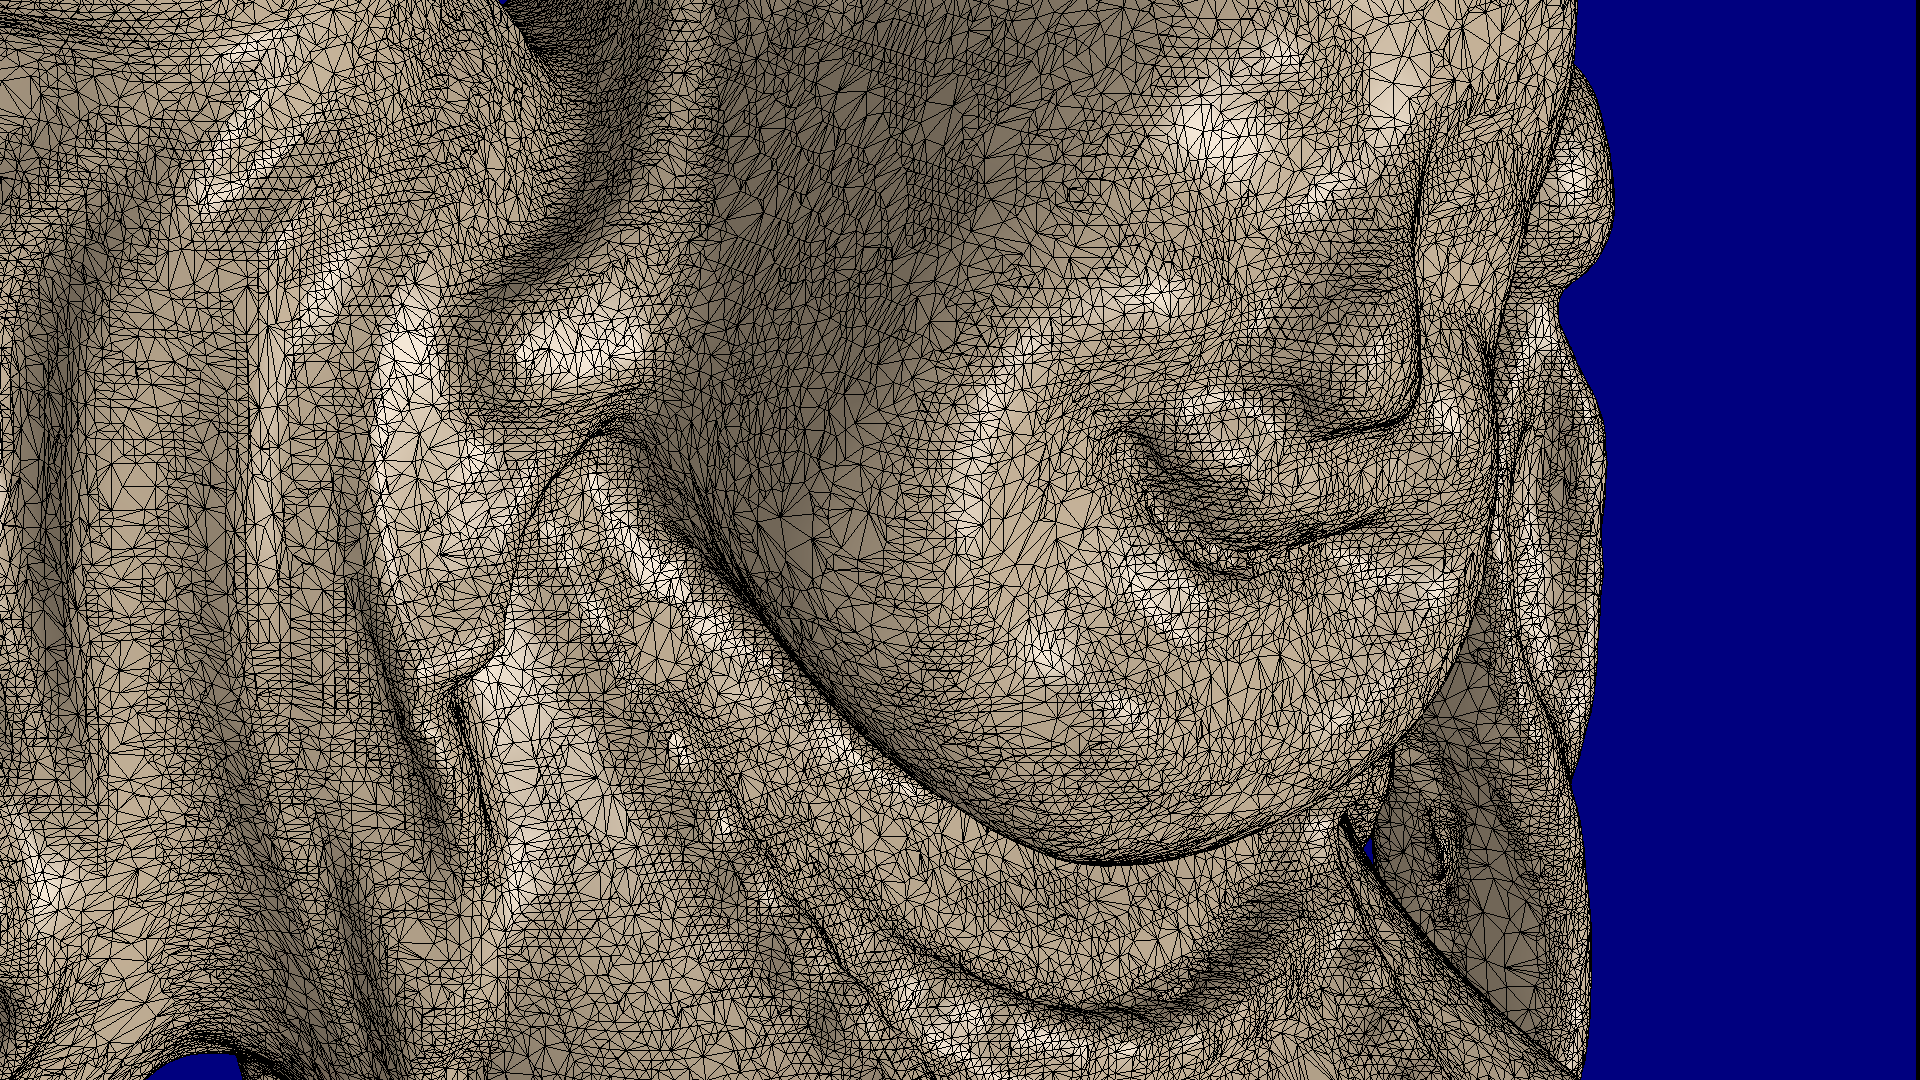
\includegraphics[width=0.80\textwidth]{fig/Buddha2.png}
	\caption{Eine Rastergrafik}
	\label{fig:exampleFigure}
\end{figure}


Bild- bzw. Tabellen-Beschriftungen sollten m�glichst informativ sein. Aus der Beschreibung sollte die Bedeutung der Abbildung vollst�ndig hervorgehen, so dass der Haupttext zum Verst�ndnis nicht notwendigerweise gelesen werden muss. 

\newpage
\section{Beispiel f�r die Darstellung von Algorithmen}

Algorithmus \ref{algo:algorithmSCAN} zeigt ...

\begin{algorithm}[htpb]
	\textit{Phase 1: Reduktion}\\
	\texttt{for} $d := 0$ \texttt{to} $log_2 n - 1$ ~\texttt{in parallel do}\\
	\hspace{5mm}\texttt{for} $k := 0$ \texttt{to} $n - 1$ \texttt{by} $2^{d+1}$ ~\texttt{in parallel do}\\
	\hspace{10mm}$x[k + 2^{d + 1} - 1] := x[k + 2^d - 1] + x [k + 2^{d + 1} - 1]$\\
	\textit{Phase 2: Propagation}\\
	\texttt{for} $d := log_2 n$ \texttt{to} $0$ ~\texttt{in parallel do}\\
	\hspace{5mm}\texttt{for} $k := 0$ \texttt{to} $n - 1$ \texttt{by} $2^{d+1}$ ~\texttt{in parallel do}\\
	\hspace{10mm}$t := x[k + 2^d - 1]$\\
	\hspace{10mm}$x[k + 2^d - 1] := x [k + 2^{d + 1} - 1]$\\
	\hspace{10mm}$x[k + 2^{d + 1} - 1] := t + x [k + 2^{d + 1} - 1]$\\
	\caption{Pseudocode der zwei Phasen vom SCAN-Algorithmus \cite{bib:SCAN}.}
	\label{algo:algorithmSCAN}
\end{algorithm}

\section{Beispiel f�r die Darstellung von Quellcode-Ausz�gen}

dies ist \verb+'+ \LaTeX

Listing \ref{lst:VBOkontrolle} zeigt ...
\lstinputlisting[language=Python, float=htpb, caption={Pseudocode f�r die Kontrolle der VBOs}, label=lst:VBOkontrolle, captionpos=b, keywordstyle=\bfseries\color{black}]{code/test.py}


Listing \ref{lst:VBOkontrolle} zeigt ...
\lstinputlisting[language=Python, style=customc, float=htpb, caption={Pseudocode f�r die Kontrolle der VBOs}, label=lst:VBOkontrolle, captionpos=b, keywordstyle=\bfseries\color{black}]{code/test.py}


Listing \ref{lst:VBOkontrolle} zeigt ...
\lstinputlisting[language=Python, style=customc, float=htpb, caption={Pseudocode f�r die Kontrolle der VBOs}, label=lst:VBOkontrolle, captionpos=b, keywordstyle=\bfseries\color{black}]{code/test2.py}


\section{Hier ein uml diagramm}
\begin{tikzpicture}
\umlemptyclass[width=15ex]{class20}
\umlemptyclass[y=2, width=30ex]{class40}
\end{tikzpicture}


\section{hier kommt pstricks}

\begin{figure}[h]
\centering
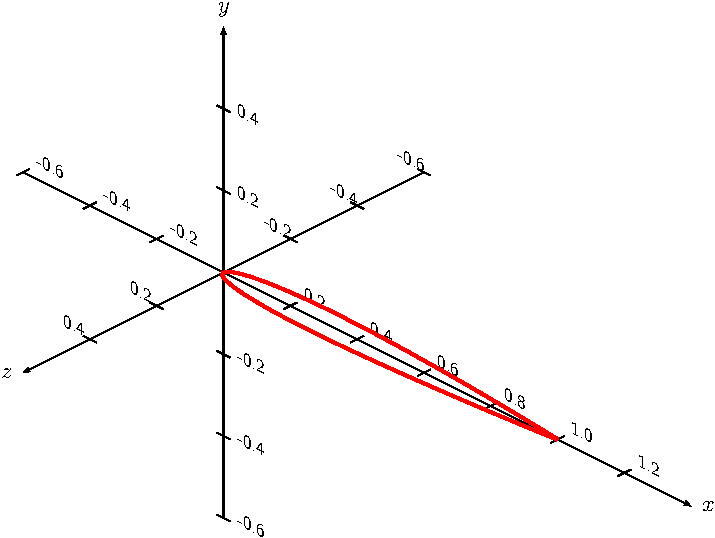
\includegraphics[width=0.7\linewidth]{tikz/Airfoil-crop}
\caption{Mein erster Funktionsplot PSTricks}
\end{figure} %% --> Leerzeile danach wichtig

\begin{figure}[h]
\centering
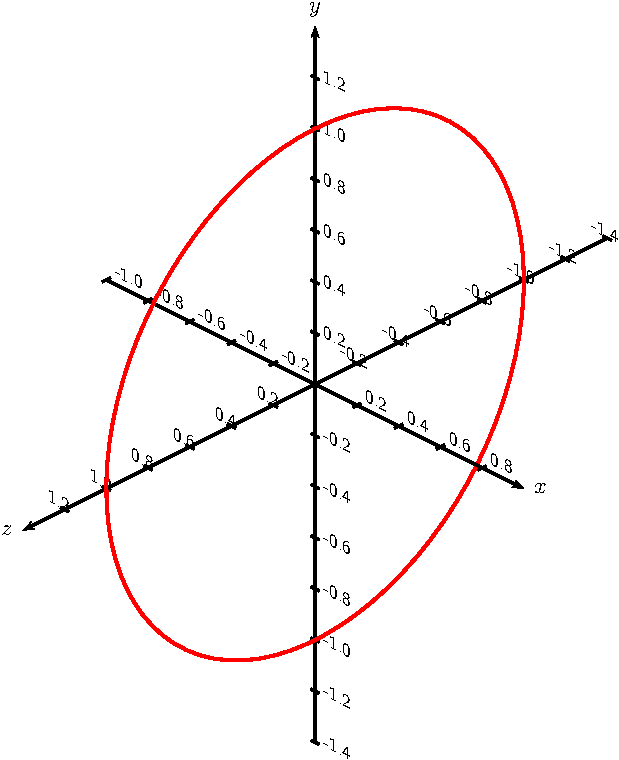
\includegraphics[width=0.7\linewidth]{tikz/Fuselage-crop}
\caption{Mein erster Funktionsplot PSTricks}
\end{figure} %% --> Leerzeile danach wichtig

%\newpage
%\newpage\thispagestyle{empty}\hspace{1em}\newpage
\chapter{Ergebnisse und Evaluation}
In diesem Kapitel sollen die Ergebnisse dieser Diplomarbeit diskutiert werden. 




%\newpage
%\newpage\thispagestyle{empty}\hspace{1em}\newpage
\chapter{Zusammenfassung und Ausblick}
In diesem Kapitel sollen zun�chst die erreichten Ziele diskutiert und abschlie�end ein Ausblick auf m�gliche, weiterf�hrende Arbeiten gegeben werden.

\newpage
\pagenumbering{Roman}
\setcounter{page}{1}

\nocite{*}%Auch nicht-zitierte BibTeX-Eintr�ge werden angezeigt.
\bibliography{Literaturverzeichnis}
\bibliographystyle{eg-alpha}
\newpage
\newpage\thispagestyle{empty}\hspace{1em}\newpage
\chapter*{Abk�rzungsverzeichnis}
\begin{acronym}[PM]
 %Sorgt daf�r, dass zwischen den Eintr�gen kein Abstand ist und das Verzeichnis kompakt dargestellt wird.
 \setlength{\itemsep}{-\parsep}
 \acro{ALU}{Arithmetic Logic Unit}
 \acro{BTF}{Bidirektionalen Textur Funktion}
 \acro{CPU}{Central Processing Unit}
 \acro{CU}{Control Unit}
 \acro{CUDA}{Compute Unified Device Architecture}
 \acro{FLOPs}{Floating Point Operations Per Second}
 \acro{FPU}{Floating Point Unit}
 \acro{GPGPU}{General Purpose Compution on Graphics Processing Unit}
 \acro{GPU}{Graphics Processing Unit}
 \acro{HLOD}{Hierarchische Level of Detail}
 \acro{IFS}{Indexed-Face-Set}
 \acro{LOD}{Level of Detail}
 \acro{MIMD}{Multiple Instruction Multiple Data}
 \acro{OpenCL}{Open Computing Language}
 \acro{OpenGL}{Open Graphics Library}
 \acro{PCAM}{Partitionierung Kommunikation Agglomeration Mapping}
 \acro{PM}{Progressive Meshes}
 \acro{SFU}{Spezial Funktion Units}
 \acro{SIMD}{Single Instruction Multiple Data}
 \acro{SIMT}{Single Instruction Multiple Threads}
 \acro{SLI}{Scalable Link Interface}
 \acro{SP}{Streaming-Prozessoren}
 \acro{SM}{Streaming-Multiprozessoren}
 \acro{TPC}{Textur Prozessor Clustern}
 \acro{VBO}{Vertex Buffer Object}

 
\end{acronym}

%Abk�rzungsverzeichnis im Inhaltsverzeichnis anzeigen
\addcontentsline{toc}{chapter}{Abk�rzungsverzeichnis} 
%Abbildungsverzeichnis
\newpage\thispagestyle{empty}\hspace{1em}\newpage
\listoffigures
%Tabellenverzeichnis
\listoftables
%Liste von Algorithmen
\newpage\thispagestyle{empty}\hspace{1em}\newpage
\markboth{Liste der Algorithmen}{Liste der Algorithmen}
\phantomsection
\addcontentsline{toc}{chapter}{Liste der Algorithmen}
\listofalgorithms
%Liste von Code
\newpage\thispagestyle{empty}\hspace{1em}\newpage
\markboth{Listings}{Listings}
\phantomsection
\addcontentsline{toc}{chapter}{Listings}
\lstlistoflistings
%Anhang
\newpage
\newpage\thispagestyle{empty}\hspace{1em}\newpage
\appendix
\chapter{Anhang}\label{chp:AnhangA}
\section*{Thema 1}\label{sec:AnhangA1}

Beispiel f�r einen Anhang

\section*{Thema 2}\label{sec:AnhangA2}

%Danksagung
\chapter*{Danksagung}
Hiermit m�chte ich mich besonders bei Prof. Dr. XXXX, Prof. Dr. xxxx, Dipl. Inf. xxxx und Dipl. Inf. xxx f�r die Betreuung meiner Arbeit, hilfreiche Diskussionen und viel Geduld bei zahlreichen Fragen bedanken.
\end{document} 